\begin{figure}[t]
  \centering
  \vspace{0.25cm}
  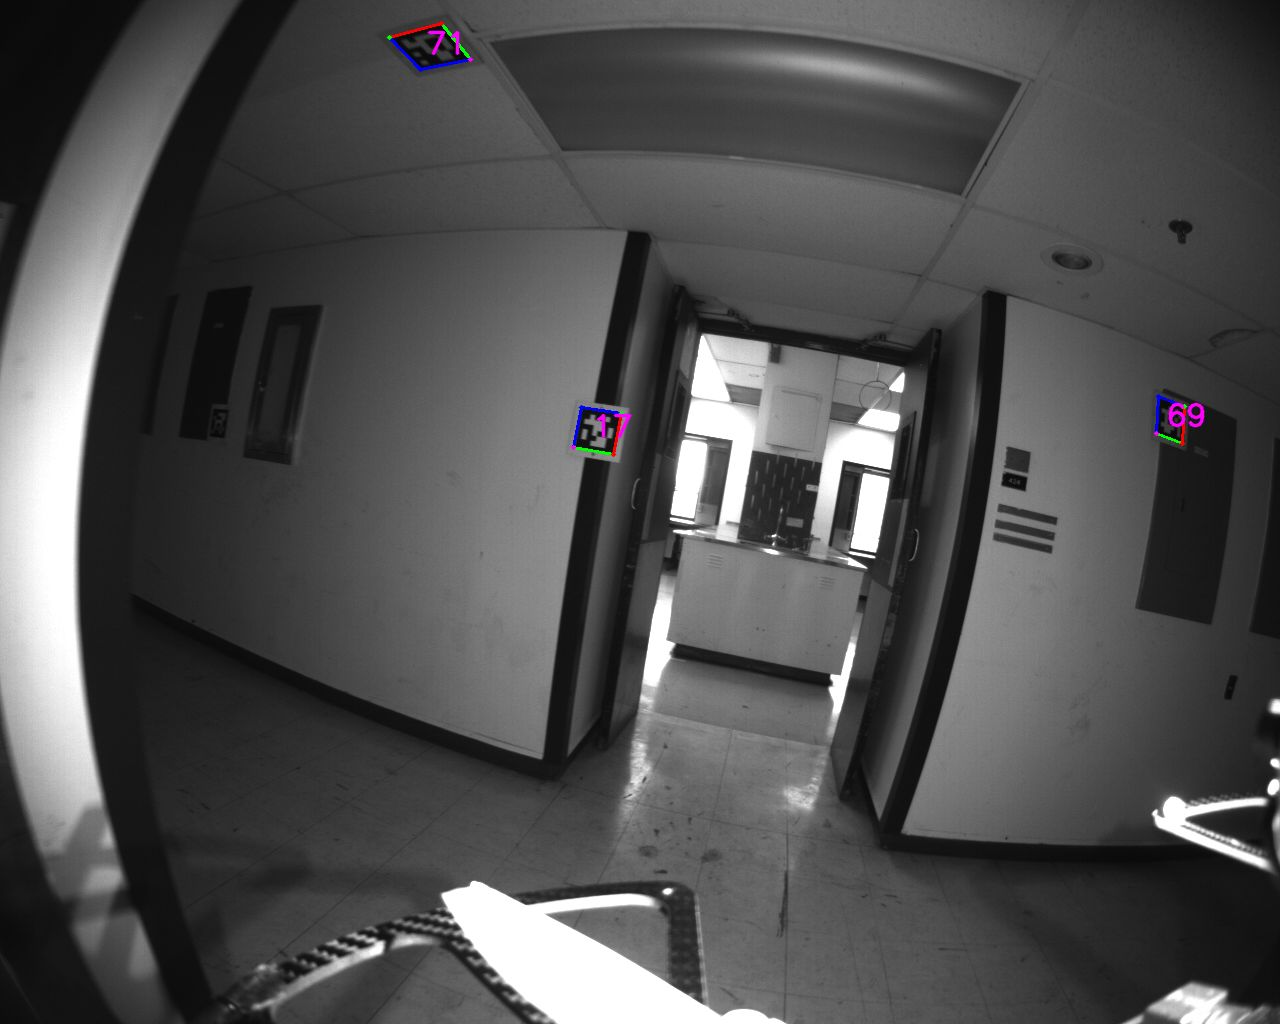
\includegraphics[width=0.65\columnwidth]{corridor_ovc.png}
  \caption{View from the left camera of an Open Vision
    Computer. Detected AprilTags are shown in color.}
  \label{fig:corridor_ovc}
\end{figure}
\section{Application Example}
\label{sec:application}
We illustrate the versatility of TagSLAM by showing how it can be used
to achieve loop closure for VIO. The synchronized images and IMU data
that serve as input for the VIO are collected with an Open Vision
Computer \cite{quigley2018}. During 13 minutes, a total of 15595
stereo frames are recorded at 20Hz along the 630m long trajectory
through the rooms of an abandoned chemical
laboratory. Fig.\ \ref{fig:corridor_ovc} shows an example image of
some of the 57 tags that are strategically placed along the
corridor. Their poses are deterimined from the wall orientations and
from laser distance measurements with a Leica Disto D3a. The odometry
is computed with the stereo VIO algorithm as described in
Ref. \cite{sun2018} but, running offline with abundant CPU resources
available, we use a larger number of visual feature points to improve
drift.

Fig.\ \ref{fig:loop_closure} shows the trajectories for VIO (cyan),
loop-closed TagSLAM (magenta), and stereo ORB-SLAM2
\cite{murartal2017} (yellow). The tag locations are visible in the map
as well. All trajectories start at the same point at the bottom of
the map, but only the TagSLAM trajectory returns correctly to the
starting point. Both VIO and ORB-SLAM2 exhibit drift, and evidently
ORB-SLAM2 does not achieve loop closure. This is not surprising since
the hallway images look very different while returning.  By combining
tag projection factors from the camera images with relative pose
factors from the odometry, TagSLAM by design closes the loop.

\begin{figure}[ht]
  \centering
  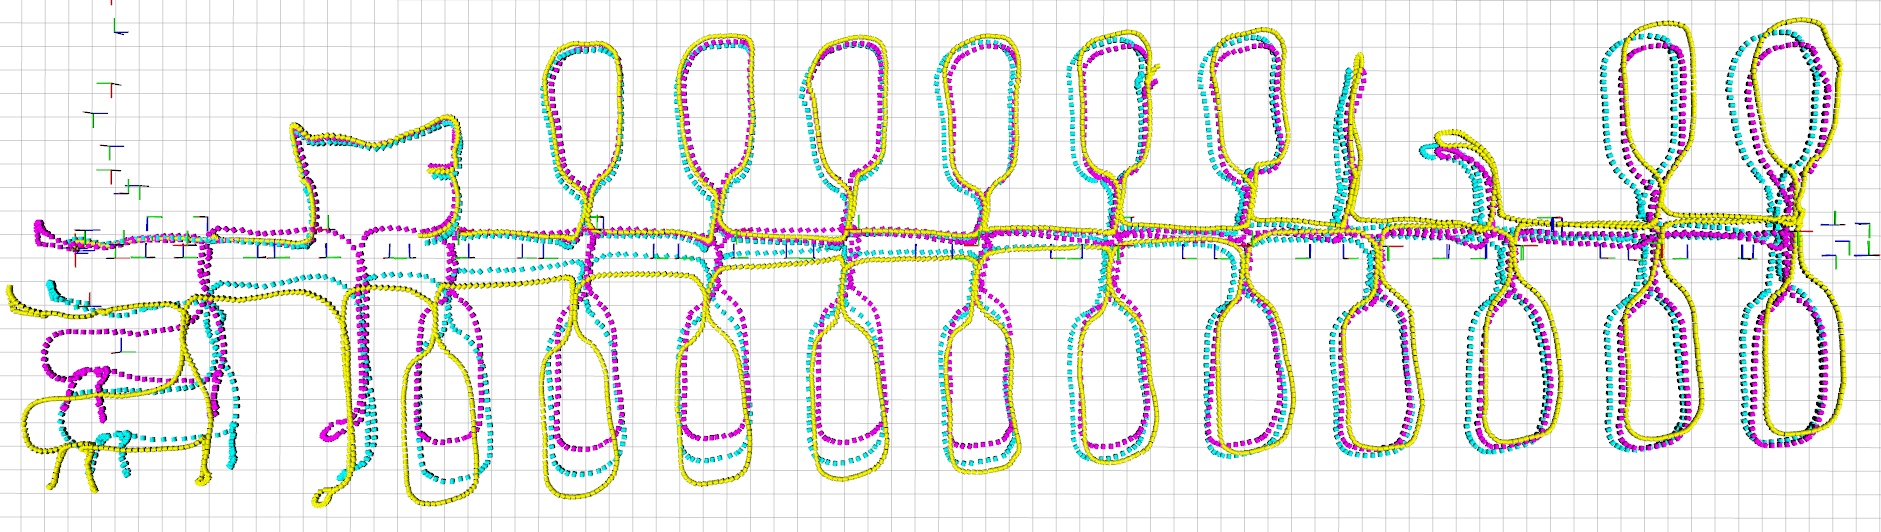
\includegraphics[angle=90, width=0.5\columnwidth]{loop_closure_building_227.png}
  \caption{Trajectory using {\color{cyan} VIO}, {\color{magenta} TagSLAM},
    and {\color{yellow} ORB-SLAM2}. The grid cell size is 1m.}
  \label{fig:loop_closure}
\end{figure}
Creating and incrementally optimizing the graph upon factor insertion
takes 188s on an Intel i9-9900K 3.6GHz CPU, which is an average
performance of about 12ms per frame. A final full (non-incremental)
graph optimization adds another 4.3s to the total processing
time. While 12ms time per frame seems to indicate the possibility of
running in real time, individual frames can take longer to process,
depending on iSAM2 relinearization. As the graph grows over time, so
does the CPU load, and individual frames can take as much as
260ms. However, for situations where there already is a trusted map of
tag poses available, TagSLAM can be configured to retain only the last
two time steps in the graph, making it suitable for real-time
operation.

